\documentclass[a4paper,12pt]{article}
\usepackage[utf8]{inputenc}
\usepackage[T1]{fontenc}
\usepackage{geometry}
\usepackage{xcolor}
\usepackage{pdfpages}
\usepackage{graphicx}
\usepackage{subcaption}

\usepackage[
    colorlinks=true,
    linkcolor=.,
    urlcolor=blue,
    citecolor=.
]{hyperref}

\usepackage{listings}
\lstdefinelanguage{riscv}{
  alsoletter=.,
  morekeywords=[1]{add, sub, lw, sw, beq, bne, jal, jalr, lui, auipc, sll, srl, sra},
  morekeywords=[2]{x0, x1, x2, x3, x4, x5, x6, x7, x8, x9, x10, x11, x12, x13, x14, x15, x16, x17, x18, x19, x20, x21, x22, x23, x24, x25, x26, x27, x28, x29, x30, x31},
  morekeywords=[3]{.data, .text, .globl, .align, .word},
  sensitive=true,
  morecomment=[l]{//},
  morestring=[b]",
}

\lstset{
  language=riscv,
  basicstyle=\ttfamily\small,
  numbers=left,
  numberstyle=\tiny,
  breaklines=true,
  frame=single,
  keywordstyle=[1]\color{blue}\bfseries,
  keywordstyle=[2]\color{teal},
  keywordstyle=[3]\color{orange}\bfseries,
  commentstyle=\color{gray}\itshape,
  stringstyle=\color{red},
}

\usepackage{parskip}
\geometry{margin=2.5cm}

\title{\textbf{Relazione RISC-V LinkedList}}
\author{Claudio Raimondi\\Matricola: 7158162\\claudio.raimondi@edu.unifi.it\\
Corso: Architettura degli Elaboratori\\
Docente: Prof. Zoppi}
\date{Data: 3 Giugno 2025}

\begin{document}

\maketitle
\tableofcontents
\thispagestyle{empty}
\newpage
\setcounter{page}{1}

\section{Overview generale}

\subsection{Obiettivi del progetto}

Il progetto consiste nell'implementazione di una \textbf{linked list} in assembly \textbf{RISC-V} 32-bit. 
La lista supporta operazioni di \textbf{inserimento}, \textbf{cancellazione}, \textbf{ordinamento}, \textbf{stampa} e \textbf{inversione} su elementi di tipo intero, ed è progettata per essere il più efficiente possibile mantenendo allo stesso tempo una buona modularità.

\subsection{Approccio ed Ambiente di sviluppo}

Per semplificare lo sviluppo ed il testing ho svolto il ruolo del compilatore: sviluppando prima un progetto funzionante in \textbf{C}, e successivamente traducendolo meticolosamente in assembly RISC-V.
In questo modo ho ridotto al minimo la possibilità di verificarsi di errori umani, e ho potuto apprendere il punto di vista del compilatore.

\subsection{Uso della memoria e dei registri}

Per evitare conflitti tra registri, ho seguito regole di convenzione sull'uso dei registri, in particolare:
\begin{itemize}
  \item \texttt{a0-a7} sono utilizzati per i parametri delle funzioni e per il valore di ritorno. (\texttt{a0} è il valore di ritorno e \texttt{a7} è utilizzato per le chiamate di sistema)
  \item \texttt{s0-s11} sono riservati per il \emph{chiamante}.
  \item \texttt{t0-t6} sono utilizzati per variabili temporanee e si assume che siano disponibili per l'uso dal \emph{chiamato}.
  \item \texttt{sp} è il puntatore allo stack.
  \item \texttt{ra} è il registro dell'indirizzo di ritorno.
  \item \texttt{zero} è il registro che contiene sempre il valore zero.
\end{itemize}

Inoltre dove necessario ho salvato i registri utilizzati nello stack, e li ho ripristinati al termine della funzione.

\subsection{Design}

Per rendere il codice il più modulare possibile, e per semplificare il \textbf{parsing}, ho adottato un approccio con array di funzioni, che in assemly si traduce come un array di indirizzi ad etichette:

\begin{lstlisting}[language=riscv]
list_functions:
  .word list_add
  .word list_del
  .word list_print
  .word list_sort
  .word list_rev
\end{lstlisting}

\section{Funzioni chiave}

\subsection{Parsing}

Il parsing dell'input è stato implementato in 3 fasi:
\begin{itemize}
    \item \textbf{Tokenizzazione}: l'input viene diviso in-place in token, sostituendo i delimitatori con il carattere '\texttt{\textbackslash0}'.
    \item \textbf{Sanificazione}: per ogni token, viene verificato che corrisponda ad un comando valido, altrimenti viene ignorato.
    \item \textbf{Esecuzione}: per ogni token valido, viene chiamata la funzione corrispondente nell'array.
\end{itemize}

\subsection{Add}

La funzione \texttt{list\_add} alloca e aggiunge un nuovo nodo in coda alla lista.
Grazie al puntatore alla coda, l'inserimento è scalabile e sarà sempre costante con complessità $O(1)$.
La chiamata a \texttt{malloc} non è gestita dal kernel come in C, ma deve essere implementata manualmente.

\subsection{Malloc}

Per implementare la funzione di allocazione dinamica della memoria, ho simulato un heap tramite una regione di memoria predefinita, che viene gestita tramite una free-list.

\begin{lstlisting}[language=riscv]
.data

node_size: .byte 5
max_nodes: .byte 30

mempool: .space 150
free_list: .space 30
\end{lstlisting}

Sapendo a priori la dimensione massima della lista, e la dimensione di ogni nodo, ho allocato un'area di memoria di 150 byte, che contiene 30 nodi da 5 byte ciascuno.
La \texttt{free\_list} invece è un array che contiene gli indici dei nodi liberi.

Per la ricerca vera e propria del primo nodo libero, per mantenere una certa semplicità ho optato per una ricerca lineare con complessità $O(n)$.

\subsection{Sort}

Per la funzione di ordinamento ho scelto l'algoritmo \textbf{Merge Sort} per 2 motivazioni principali:
\begin{itemize}
    \item complessità sempre $O(n \log n)$, senza degenerare.
    \item mancanza di alternative per una lista concatenata, che non permette l'accesso casuale agli elementi.
\end{itemize}

Per la ricerca del punto medio della lista, ho utilizzato la tecnica dei \textbf{puntatori lento e veloce}, che dimezza la complessità rispetto ad una ricerca lineare:

\begin{lstlisting}[language=C]
t_node *slow = *head;
t_node *fast = *head;
while (fast->next && fast->next->next)
{
  slow = slow->next;
  fast = fast->next->next;
}
t_node *mid = slow->next;
\end{lstlisting}

La funzione merge è stata implementata in modo ricorsivo e totalmente \emph{branchless} grazie all'utilizzo di variabili booleane come indici di array:

\begin{lstlisting}[language=C]
while ((a != NULL) & (b != NULL))
{
  idx = (b->data < a->data);

  chosen = nodes[idx];
  current->next = chosen;
  current = chosen;
  nodes[idx] = chosen->next;
  a = nodes[0];
  b = nodes[1];
}
\end{lstlisting}

Questa, anche se sembra una scelta facile, in realtà potrebbe essere subottimale rispetto ad una soluzione branchy, a causa della latenza delle operazioni di load e store. In conclusione però, la predittibilità della versione branchless rimuove il rischio di branch mispredictions che aggiungevano ben più stalli alla pipeline.

\section{Analisi quantitativa e ottimizzazione}

\subsection{Cache}

Per ottimizzare la località spaziale delle istruzioni, così da ridurre il numero di cache miss, le ho riordinate tenendo in mente diversi fattori:

\begin{itemize}
    \item le funzioni chiamate più frequentemente hanno priorità più alta
    \item funzioni che si chiamano a vicenda sono vicine tra loro
    \item l'utente è più propenso a chiamare le funzioni \texttt{add} e \texttt{print}
    \item il branch predictor può favorire salti all'indietro
\end{itemize}

Eseguendo un semplice benchmark con il comando:

\begin{center}
\texttt{ADD(1)} $\sim$ \texttt{SORT} $\sim$ \texttt{REV} $\sim$ \texttt{DEL(1)} $\sim$ \texttt{ADD(1)} $\sim$ \texttt{PRINT}
\end{center}

otteniamo un \emph{cache miss} rate di circa 8\% per le \textbf{istruzioni}, e 2\% per i \textbf{dati}, indipendentemente dal tipo di cache:

\begin{figure}[h]
  \centering
  \begin{subfigure}[b]{0.45\textwidth}
    \centering
    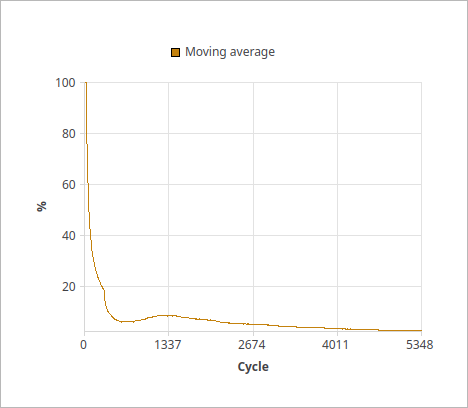
\includegraphics[width=\textwidth]{assets/data_cache_miss.png}
    \caption{Data Cache Miss}
    \label{fig:data_cache_miss}
  \end{subfigure}
  \hfill
  \begin{subfigure}[b]{0.45\textwidth}
    \centering
    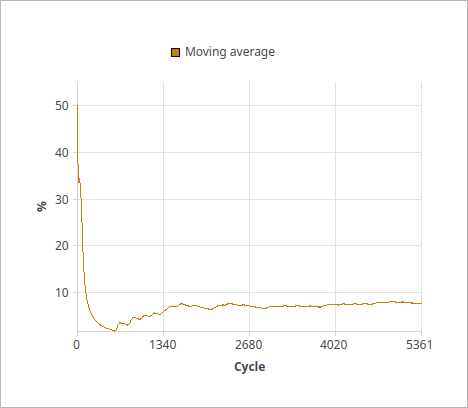
\includegraphics[width=\textwidth]{assets/instruction_cache_miss.png}
    \caption{Instruction Cache Miss}
    \label{fig:instruction_cache_miss}
  \end{subfigure}
\end{figure}

\subsection{Branches}

Per ridurre al minimo il numero di branch mispredictions, e quindi di stalli, ho utilizzato tecniche branchless:

\begin{itemize}
  \item sacrificare lo short-circuiting utilizzando \textbf{operatori bitwise} invece di operatori logici (\texttt{\&} e \texttt{|} invece di \texttt{\&\&} e \texttt{||})
  \item utilizzare variabili booleane come indici di array, come visto nella funzione \texttt{merge}
  \item moltiplicazione per 0 e 1 (condizione e condizione opposta)
\end{itemize}

In questo modo, l'intero codice ha solo 24 salti condizionati.

\section{Riferimenti}

\begin{itemize}
    \item \href{https://github.com/Raimo33/LinkedList}{Codice sorgente su GitHub}
    \item \href{https://github.com/mortbopet/Ripes}{Simulatore RIPES}
    \item \href{https://riscv.org/}{RISC-V Foundation}
\end{itemize}

\end{document}
